\documentclass{article}
\usepackage[utf8]{inputenc}
\usepackage{graphicx}
\usepackage{here}
\usepackage{amsmath}
\usepackage{amsfonts}

\title{Notes de cours\\OPT6 : Apprentissage avancé}
\author{Adrien Pavao}
\date{Novembre 2017}

\begin{document}

\maketitle

%\tableofcontents

\section{Introduction}

L'apprentissage automatique (machine learning) s'appuie sur des bases théoriques. Ce domaine évolue vite et on y trouve des théories et techniques avancées.

\begin{figure}[H]
  \centering
  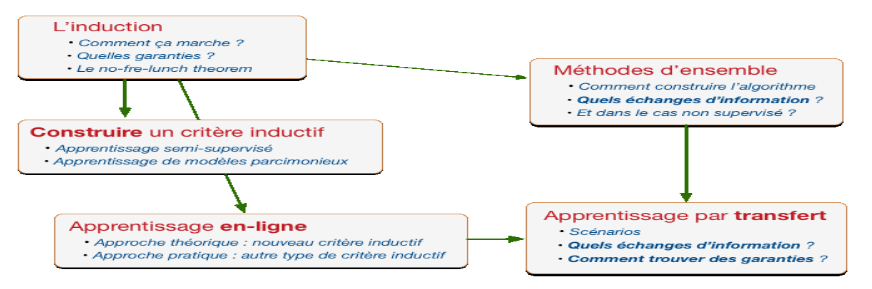
\includegraphics[scale=0.4]{outline.png}
  \caption{Les points qui seront abordés dans ce cours.}
\end{figure}

\subsection{Quelques notions}
\begin{itemize}
\item Vladimir Vapnik a posé les bases théoriques de l'apprentissage statistique\footnote{https://en.wikipedia.org/wiki/Statistical\_learning\_theory}.
\item Apprentissage PAC : Probably Approximately Correct\footnote{https://en.wikipedia.org/wiki/Probably\_approximately\_correct\_learning}.
\item \textbf{No-free-lunch theorem :} Il n'existe pas de méthode d'apprentissage qui soit meilleure qui les autres. Même performance que l'aléatoire sur l'ensemble des problèmes possibles. Si une méthode est efficace sur un problème elle sera mauvaise sur un autre. L'intégrale sur tous les problèmes est toujours la même, quelque soit la méthode. Idem pour les mesures (de distance par exemple). Les méthodes sont adaptées à des \textbf{classes} de problèmes. \textbf{Tous les algorithmes inductifs se valent.}
\item \textbf{Adversarial learning :} L'intersection entre le machine learning et la sécurité informatique.
\item \textbf{Régularisation :} Un processus consistant à ajouter de l'information à un problème pour éviter le surapprentissage. Cette information prend généralement la forme d'une pénalité envers la complexité du modèle. On peut relier cette méthode au principe du \textbf{rasoir d'Occam}. D'un point de vue bayésien, l'utilisation de la régularisation revient à imposer une distribution a priori sur les paramètres du modèle.

Une méthode généralement utilisée est de pénaliser les valeurs extrêmes des paramètres, qui correspondent souvent à un surapprentissage. Pour cela, on va utiliser une norme sur ces paramètres, que l'on va ajouter à la fonction qu'on cherche à minimiser. Les normes les plus couramment employées pour cela sont $L_1$ et $L_2$.

\item Différentes normes permettent de calculer la taille totale d'un vecteur ou d'une matrice dans un espace vectoriel. Quelques exemples courants : 

      Norme $L_0$ :
            \[ ||x||_0 = \sqrt[0]{\sum_i x_i^0} \]
      Norme $L_1$ :
            \[ ||x||_1 = \sum_i |x_i| \]
      Norme $L_2$ :
            \[ ||x||_2 = \sqrt{\sum_i x^2_i} \]
            
\item \textbf{Distance de Manhattan :} La distance entre deux points lorsque les déplacements sont faits selon un réseau ou un quadrillage. 

\begin{figure}[H]
    \begin{center} 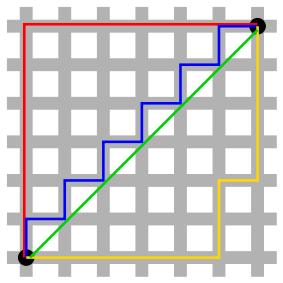
\includegraphics[scale=0.5]{manhattan.png} \end{center}
     \caption{Distance de Manhattan (chemins rouge, jaune et bleu) contre distance euclidienne en vert.}
\end{figure}

Le nom de cette distance fait sans doute référence à l'architecture en quadrillage du quartier de Manhattan, à New York.

\item Référence d'un livre intéressant : \textit{Hofstadter - "Godel, Escher, Bach".}
\item \textbf{Complexité de Kolmogorov :} Une fonction permettant de quantifier la taille du plus petit algorithme nécessaire pour engendrer un nombre ou une suite quelconque de caractères. Cette quantité peut être vue comme une évaluation d'une forme de complexité de cette suite de caractères.
\item Effets de séquences : Une séquence d'information influe sur le résultat de l'induction (à préciser).
\item L'algorithme d'apprentissage du perceptron converge si les données sont linéairement séparables. Cette convergence est en nombre fini d'étapes et ce nombre est indépendant du nombres d'exemples, de la distribution des exemples, et quasiment pas de la dimension de l'espace d'entrée. Il dépend de la marge de séparation des nuages de points et du diamètre de la boule (à préciser).
\item \textbf{L'espace des versions :} Toutes les hypothèses correctes (qui ne font pas d'erreurs) d'après les données d'apprentissage.
\end{itemize}

\section{Induction}

On déduit à partir d'un échantillon.

\begin{enumerate}
\item Espace d'hypothèse H.
\item Critere inductif $ S \times h \in H \rightarrow $ Score $\in \mathbb{R}$. Par exemple minimiser le taux d'erreur.
\item Methode d'exploration de H.
\end{enumerate}

On ne dispose pas de théorie bien établie de l'induction (exemple Fibonacci).

\subsection{Différents types d'apprentissage}
\begin{itemize}
\item \textbf{Descriptif :} Non supervisé. On cherche des régularités dans les données. On ne souhaite pas extrapoler, on ne s'interesse qu'à l'échantillon de données dont on dispose. La "matière noire" de l'apprentissage.
\item \textbf{Prédictif :} Supervisé. L'échantillon de données sert à apprendre une hypothèse sur les données pour prédire ensuite sur de nouvelles données. On cherche des corrélations entre les données.
\item \textbf{Prescriptif :} On cherche des \textbf{causalités}. Il s'agit d'une tâche difficile.
\end{itemize}

Les frontières entre ces types d'apprentissage peuvent être floues, on peut par exemple commencer par une description des données pour les comprendre avant de faire un modèle prédictif.

\subsection{Différentes méthodes d'apprentissage}

Dans ce cours nous allons aborder différentes méthodes d'apprentissage.

\begin{itemize}

\item Méthodes d'ensemble : Combiner plusieurs hypothèse (exemple : boosting).

\item Supervisé. La méthode classique d'apprentissage passif est appelé \textit{apprentissage batch}. C'est la technique la plus utilisée aujourd'hui.

\item L'induction :
    \begin{itemize}
    \item Apprentissage semi supervisé 
    \item Apprentissage de modèles parcimonieux (peu de paramètres).
    \end{itemize}

\item Apprentissage en ligne (online learning) : Les données arrivent en cours de route.

\item \textbf{Apprentissage par transfert :} Cela vise à transférer des connaissances d'une ou plusieurs tâches sources vers une ou plusieurs tâches cibles. On peut le voir comme la capacité d’un système à reconnaître et appliquer des connaissances et des compétences, apprises à partir de tâches antérieures, sur de nouvelles tâches ou domaines partageant des similitudes.

\end{itemize}

\subsection{Types de biais}

L'induction necessite d'être biaisé, d'avoir une preference pour certaines hypothèses, de ne pas connaitre toutes les fonctions possibles. Un biais classique et très humain est la préférence des hypothèses les plus simples (rasoir d'Ockham).

\begin{itemize}
\item \textbf{Biais de représentation (déclaratif) :} On ne peut représenter qu'un petit nombre de fonctions possibles. Le langage dans lequel on exprime le problème ne me permet pas de tout représenter.
\item \textbf{Biais de recherche (procédural) :} La procédure de recherche avantage certaines hypothèses. Par exemple on reste proche de notre point initial de recherche dans l'espace des fonctions possibles.
\end{itemize}

Souvent un peu des deux.

\subsection{Risques}

On distingue deux types de risques :

\begin{itemize}
\item \textbf{Risque réel} (ce que l'on veut minimiser). La performance à venir si j'utilise l'hypothèse h. Cela prend la forme d'une espérance de coût d'usage de h. Le risque réel (loss function) : 
\[ R(h) = \displaystyle \int_X^Y l(h(x), y) p(x, y) \mathrm{d}x \mathrm{d}y \]

La meilleure hypothèse est $k^* = Argmin R(h)$ avec $h \in H$. En d'autres termes, on cherche l'hypothèse qui minimise le risque réel. $l$ est la métrique d'évaluation et $p$ la loi de probabilité hypothétique ayant générée la distribution des données.
\item \textbf{Risque empirique}. Puisque l'on cherche la loi de probabilité, on ne la connait pas et on ne peut donc pas s'en servir pour calculer le risque, en pratique. On calcul donc le risque empirique : 
\[ \hat{R}(h) = \frac{1}{m} \sum_{i=1}^m l(h(x_i), y_i) \]
C'est donc la moyenne des distances entre les prédictions avec h et les valeurs réelles des données. \^h est l'hypothèse minimisant le risque empirique. 
\end{itemize}

On cherche les liens entre toutes ces notions.

\subsubsection*{Pour Vladimir Vapnik}

Plutôt que de minimiser le risque empirique : 
\begin{itemize}
\item Pour une hypothèse h : $ P_{S \sim P_{XY}} (\hat{R}(h) = 0 \wedge R(h) > \epsilon ) $
\end{itemize}
On ne veux pas d'une hypothèse qui paraisse bonne mais qui soit en réalité mauvaise. Le principe de minimisation du risque empirique n'est sain que s'il y a des contraintes sur l'espace des hypothèses.

(formule et principe de consistance universelle ?)

\section{Transduction}

On ne s'interesse qu'à un point. Le nombre de données requises pour tirer une conclusion n'est plus influencé par le nombre de dimension. On parle de \textbf{transductive learning}.
\begin{itemize}
\item Transduction : Cas d'induction limite (une question).
\item Analogie : Cas de transduction limite (un exemple).
\end{itemize}

\section{Possibilités d'apprendre}

\subsection{Perceptron}

\begin{enumerate}
\item On suppose que l'ensemble des hypothèses H est fini.
\item \textbf{Cas réalisable :} $ \exists h \in H tq R(h) = 0 $ ($ \ne 0 \rightarrow$ cas non-réalisable.)
\item S est supposé tiré \textit{i.i.d.}
\end{enumerate}


\subsection{Dimension Vapnik-Chervonenkis}

La $d_{VC}$ est la taille du plus grand ensemble de points tirés aléatoirement que l'on peut pulvériser, c'est-à-dire que l'on peut étiqueter n'importe comment en utilisant une hypothèse de H.

$d_{VC}(H)$ donne une idée de l'expressivité du modèle (de l'espace de réalisation).

\begin{figure}[H]
  \centering
  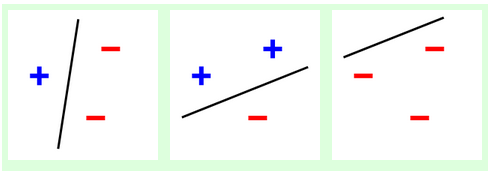
\includegraphics[scale=0.4]{dimension_vc1.png}
  \caption{Pulvérisation de 3 points}
\end{figure}

\begin{figure}[H]
  \centering
  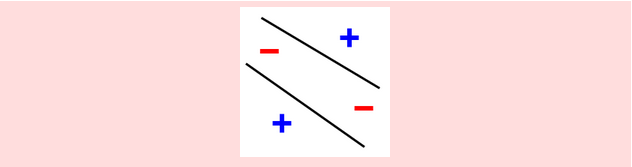
\includegraphics[scale=0.4]{dimension_vc2.png}
  \caption{Lorsqu'il y a 4 points, la pulvérisation est impossible}
\end{figure}

$d_{VC}$ de l'ensemble des droites = 3.

\subsection{Apprentissage faible et fort}

\begin{itemize}
\item \textbf{Apprenant faible :} Erreur réelle $< \frac{1}{2} - \gamma$, $\gamma > 0$. Typiquement un decision stump.
\item \textbf{Apprenant fort :} On peut être infiniment exigeant. $\forall \epsilon$, $\forall \delta$, avec suffisamment d'exemples, A trouvera une hypothèse h d'erreur réelle $< \epsilon$ dans plus de $1 - \delta$ des cas (échantillons). Dans le cas réalisable.
\end{itemize}

\subsection{Borne sur le risque réel}

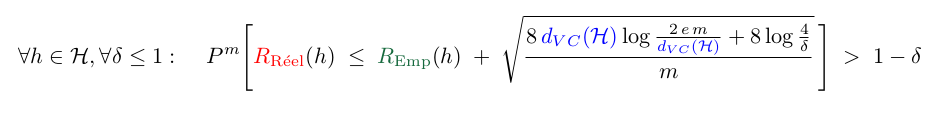
\includegraphics[scale=0.4]{risk_bound.png}

\section{Apprentissage à partir de flux de données}

\subsection{Flux de données}

Un flux de données, ou data stream, est une séquence de mesures 
\begin{align}
 S = <x_1, x_2, ..., x_t, ...> \\
 S = <(\underbrace{x_1}_{\hat{y}_1}, y_1),(\underbrace{x_2}_{\hat{y}_2}, y_2), ..., (\underbrace{x_t}_{\hat{y}_t}, y_t), ...>
\end{align}

\subsection{Plusieurs séquences}

\begin{itemize}
\item Clustering
\item Classification supervisée
\end{itemize}

Nécessite la définition d'une distance appropriée. On ne peut pas permuter les éléments de la séquence sans modifier le problème. \\
Exemple : Génomes, distances d'édition, programmation dynamique.

\subsection*{Tâches classiques}

\subsection{Prédiction (une séquence)}

\begin{itemize}
\item ARIMA : régression linéaire

 
\item Chaines de Markov
\item HMM (Modèle de Markov Caché)

\item Grammaires
\item Réseaux de neurones récurrents

\end{itemize}

Données discretisées (peu de symbols) dans le cas des chaines de Markov et des HMM.

\subsection{Apprentissage en ligne (online learning)}

Apprentissage en cours de route.

L'apprentissage par renforcement peut être vu comme une sorte d'apprentissage en ligne.

\begin{enumerate}
\item Scénario :

\[ \underbrace{x_1 \rightarrow \hat{y}_1 = h_{1}(\vec{x_1}) \leftrightarrow y1}_{h_2} \]
\[ \underbrace{x_2 \rightarrow \hat{y}_2 = h_{2}(\vec{x_2}) \leftrightarrow y2}_{h_h} \]
% mmh ...

\item Motivations pour ce scénario
\begin{itemize}
\item Cadre Anytime : même en environnement stationnaire
\item Environnement non stationnaire.
      \begin{itemize}
      \item Types de changements : Sur $P_x$ : \textbf{covariate shift}.
      \item Sur $P_{Y|X}$ : \textbf{concept drift} (dérive de concept).
      \end{itemize}
\item Données très volumineuses.
      \begin{itemize}
      \item Adaptation de domaine (domain adaptation) : "en gros" covariate shift.
      \item Apprentissage par transfert (transfer learning) : changement de tâche.
      \end{itemize}
\end{itemize}
\end{enumerate}

\subsection{Apprentissage incrémental}

\begin{itemize}
\item Environnement stationnaire.
\item Séquence pédagogique pour apprendre un concept complexe.
\end{itemize}

\subsubsection*{Evaluation de l'apprentissage}

Comment faire en environnement non stationnaire ? On ne peux plus utiliser le risque empirique. Prequential criterion. Nombre d'erreurs de prédiction commises sur un intervalle T.

\subsubsection*{Comment réaliser l'apprentissage}

\[ A : H \times X \times Y \]
\[ (h_t, x_t, y_t) \rightarrow h_{t+1} \]

\subsection{Experts : un scénario maximaliste}

\begin{itemize}
\item La théorie de l'apprentissage en ligne (online learning theory).
\item Contre toute séquence y compris les séquences adverserielles.
\item Notion de "\textbf{comité d'experts}".
\item Ensemble de N "experts".
\item Expert : $x \rightarrow$ y.
\item Aucune hypothèse sur le fonctionnement interne des experts (statique, dynamique...)
\end{itemize}

(0 $\rightarrow$ bonne réponse, 1 $\rightarrow$ erreur)

\begin{figure}[H]
\begin{tabular}{|c|c|c|c|c|c|c|}
    \hline
    \_ & Expert 1 & Expert 2 & Expert 3 & Expert 4 & Expert 5 & Expert 6 \\
    \hline
    Exemple 1 & 1 & 0 & 0 & 1 & 0 & 1 \\
    Exemple 2 & \_ & \_ & \_ & \_ & \_ & \_ \\
    \hline 
\end{tabular}
\end{figure}

Ressemblance avec les bandits manchots. Les concepts de dilemme exploration-exploitation et de regret s'appliquent.

\subsubsection{Algorithmes gloutons}

\subsubsection*{Algorithme glouton déterministe}

On prend à chaque étape l'expert qui a fait le moins d'erreur. Déterministe car on selectionne de gauche à droite quand il y a égalité, en partant (du suivant) du dernier que l'on a pris.

\begin{figure}[H]
\begin{tabular}{|c|c|c|c|c|c|c|}
    \hline
    \_ & Expert 1 & Expert 2 & Expert 3 & Expert 4 & Expert 5 & Expert 6 \\
    \hline
    Exemple 1 & 1 & [\textbf{0}] & 0 & 1 & 0 & 1 \\
    Exemple 2 & 1 & 1 & 1 & 0 & [\textbf{0}] & 0 \\
    Exemple 3 & 1 & [\textbf{0}] & 0 & 0 & 1 & 1 \\
    \hline 
\end{tabular}
\end{figure}

Le pire cas du glouton déterministe :

\begin{figure}[H]
\begin{tabular}{|c|c|c|c|c|c|c|}
    \hline
    \_ & Expert 1 & Expert 2 & Expert 3 & Expert 4 & Expert 5 & Expert 6 \\
    \hline
    Exemple 1 & [\textbf{1}] & 0 & 0 & 0 & 0 & 0 \\
    Exemple 2 & 0 & [\textbf{1}] & 0 & 0 & 0 & 0 \\
    Exemple 3 & 0 & 0 & [\textbf{1}] & 0 & 0 & 0 \\
    \hline 
\end{tabular}
\end{figure}

\[ \underbrace{L}_{\text{Perte algo}} \leq N(L^{*}) + N - 1 \]

Si l'adversaire tire profit de sa connaissance de l'algorithme, le glouton déterministe est très catastrophique. On peut éviter ça en tirant aléatoirement. Il s'agit donc du glouton aléatoire, ou glouton non-déterministe.

\subsubsection*{Algorithme glouton aléatoire}

Pire cas : 

\[ L_{RG} \leq (ln N + 1)(L^{*}) + ln N \]

C'est bien mieux.

\subsubsection{Algorithmes de vote}

\subsubsection*{Algorithme du vote majoritaire}

\begin{itemize}
\item \textbf{Cas réalisable :} un expert aura 0 erreur sur la séquence.

A chaque erreur à l'instant t : 
\[ W_{t+1} < \frac{W_t}{2} \]
\[ L_{CR} \leq [log_2 N] \]

\item \textbf{Cas non réalisable :} A $t = 0$, $W_0 = N$.

Pour chaque expert i :
\[ w_{i}(t+1) = \begin{cases}
               w_{i}(t) \\
               \beta w_{i}(t) \\
               \beta \in [0, 1[ \\
              \end{cases}
\]

Supposons qu'une erreur soit commise à l'instant t :

\[ W(t+1) \leq \frac{W(t)}{2} + \beta \frac{W(t)}{2} \]

Après m erreurs : 

\[ W_m \leq W_0 \frac{(1 + \beta)^m}{2^m} \]

\begin{center}
Poids du meilleur expert $ = \beta^{m^{*}} $
\end{center}

\[ m \leq \frac{log_2 N + m^{*} log_2 (\frac{1}{\beta})}{log_2 \frac{2}{1 + \beta}} \]

\end{itemize}

\subsection{Approches heuristiques}

Dérive de concept (continu, des ruptures rares).

\subsubsection*{Le compromis plasticité-stabilité}

\begin{itemize}
\item \textbf{Stabilité :} Interêt à considerer un maximum de données
\item \textbf{Plasticité :} Pouvoir s'adapter si le concept change, savoir oublier.
\end{itemize}

\section{Apprentissage par transfert et adaptation de domaine}

Notations usuelles : 
\begin{itemize}
\item S : Domaine source
\item T : Domaine cible
\item $D_s (P_x^s)$ : Distribution des exemples sources
\item $D_s (P_x^T)$ : Distribution des exemples cibles
\item $h_s$ : Hypothèse apprise sur la source
\item $h_T$ : Hypothèse apprise sur la cible
\item $S_s$ : Echantillon de données sources
\item $S_T$ : Echantillon de données cibles
\end{itemize}

En vrac :

\begin{itemize}

\item Souvent, on suppose que $ |S_T| << |S_s| $.

\item La \textbf{divergence de Kullback-Leibler} est une mesure de dissimilarité entre deux distributions de probabilités P et Q.

\item Jeu pathologique : Plus on explore loin, plus on perd d'information.

\end{itemize}

\subsection{Définition et illustration}

\begin{center} Source $X_s \rightarrow y_s $ \end{center}
\begin{center} Cible $X_T \rightarrow y_T $ \end{center}
$$ X \rightarrow Y $$

\begin{figure}[H]
  \centering
  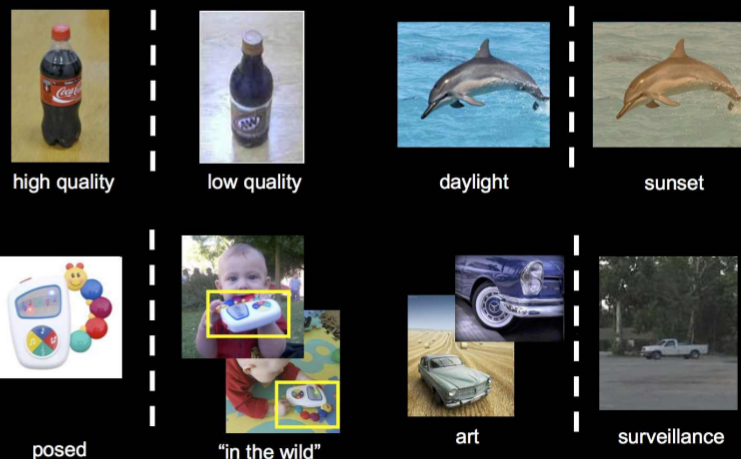
\includegraphics[scale=0.4]{domain_transfer.png}
  \caption{Exemples de transferts de domaine}
\end{figure}

Les trois grandes approches (slides 87) :

\begin{itemize}
\item Instance-based method : reweighting
\item Features-based method : find new representation spaces
\item Iterative method : adjustement
\end{itemize} 

\subsection{Une approche de l'apprentissage par transfert}

Le problème motivant le travail.
Classification précoce de série temporelles.
On va apprendre des fonctions de $ X_t \rightarrow \underbrace{X_s}_{\text{Toutes les mesures possibles}} $

On apprend des fonctions $\pi_i$ par le boosting. A la fin :

$$ H(\vec{x}_t) = signe \bigg\{ \sum_{i=1}^N \alpha_i h_s \circ \underbrace{\pi_i(\vec{x}_t)}_{\in X_s} \bigg\} $$

\end{document}




